\documentclass{article}\usepackage[]{graphicx}\usepackage[]{color}
%% maxwidth is the original width if it is less than linewidth
%% otherwise use linewidth (to make sure the graphics do not exceed the margin)
\makeatletter
\def\maxwidth{ %
  \ifdim\Gin@nat@width>\linewidth
    \linewidth
  \else
    \Gin@nat@width
  \fi
}
\makeatother

\definecolor{fgcolor}{rgb}{0.345, 0.345, 0.345}
\newcommand{\hlnum}[1]{\textcolor[rgb]{0.686,0.059,0.569}{#1}}%
\newcommand{\hlstr}[1]{\textcolor[rgb]{0.192,0.494,0.8}{#1}}%
\newcommand{\hlcom}[1]{\textcolor[rgb]{0.678,0.584,0.686}{\textit{#1}}}%
\newcommand{\hlopt}[1]{\textcolor[rgb]{0,0,0}{#1}}%
\newcommand{\hlstd}[1]{\textcolor[rgb]{0.345,0.345,0.345}{#1}}%
\newcommand{\hlkwa}[1]{\textcolor[rgb]{0.161,0.373,0.58}{\textbf{#1}}}%
\newcommand{\hlkwb}[1]{\textcolor[rgb]{0.69,0.353,0.396}{#1}}%
\newcommand{\hlkwc}[1]{\textcolor[rgb]{0.333,0.667,0.333}{#1}}%
\newcommand{\hlkwd}[1]{\textcolor[rgb]{0.737,0.353,0.396}{\textbf{#1}}}%

\usepackage{framed}
\makeatletter
\newenvironment{kframe}{%
 \def\at@end@of@kframe{}%
 \ifinner\ifhmode%
  \def\at@end@of@kframe{\end{minipage}}%
  \begin{minipage}{\columnwidth}%
 \fi\fi%
 \def\FrameCommand##1{\hskip\@totalleftmargin \hskip-\fboxsep
 \colorbox{shadecolor}{##1}\hskip-\fboxsep
     % There is no \\@totalrightmargin, so:
     \hskip-\linewidth \hskip-\@totalleftmargin \hskip\columnwidth}%
 \MakeFramed {\advance\hsize-\width
   \@totalleftmargin\z@ \linewidth\hsize
   \@setminipage}}%
 {\par\unskip\endMakeFramed%
 \at@end@of@kframe}
\makeatother

\definecolor{shadecolor}{rgb}{.97, .97, .97}
\definecolor{messagecolor}{rgb}{0, 0, 0}
\definecolor{warningcolor}{rgb}{1, 0, 1}
\definecolor{errorcolor}{rgb}{1, 0, 0}
\newenvironment{knitrout}{}{} % an empty environment to be redefined in TeX

\usepackage{alltt}
\usepackage{fullpage}
\usepackage[colorlinks=true,linkcolor=blue]{hyperref}
\usepackage{placeins}
\usepackage{subcaption}

\title{Final Project Proposal}
\author{Dominic LaRoche}
\IfFileExists{upquote.sty}{\usepackage{upquote}}{}
\begin{document}
\maketitle

\section{Introduction}
Mosquitoes are a problematic transmission vector for a number of infectious diseases in tropical and sub-tropical regions throughout the globe.  These diseases, such as malaria, can be particularly deadly for vulnerable populations with restricted access to healthcare.  One promising method for mitigating the risk of infection from mosquitoes is the use of bed nets which reduce the number of encounters with mosquitoes and the diseases they harbor.  Another method for reducing the risk of mosquito born illnesses is the use of aerial pesticides to reduce the local mosquito population. Both of the methods have been employed in Kenya in recent years.  \\

Both bed nets and aerial spraying take time and money to deploy.  Therefore, it is critical that treatments are applied to populations at the highest risk of exposure to mosquitoes and not to populations with low exposure risk.  However, it is unclear whether at risk populations are more likely to have received one of these treatments than those at lower risk for contact with mosquitoes.  The purpose of this study is to determine whether individuals with the highest risk of exposure are more likely to receive one of the  afore mentioned treatments.\\



\section{Methods}
\subsection{Data Description}
The data are composed of 3,984 households at two sites in Kenya.  These two sites represent high elevation and low elevation populations.  Both sites have had partial treatment with both bed nets and aerial spraying.  The high site has more prevalent bed net usage whereas the low site has more prevalent aerial spraying (figs. \ref{high} and \ref{low}).  A number of attributes are associated with each household including the number of occupants, the age of the occupants, and the location of the house.\\

\begin{figure}
\centering
\begin{subfigure}[b]{.48\textwidth}
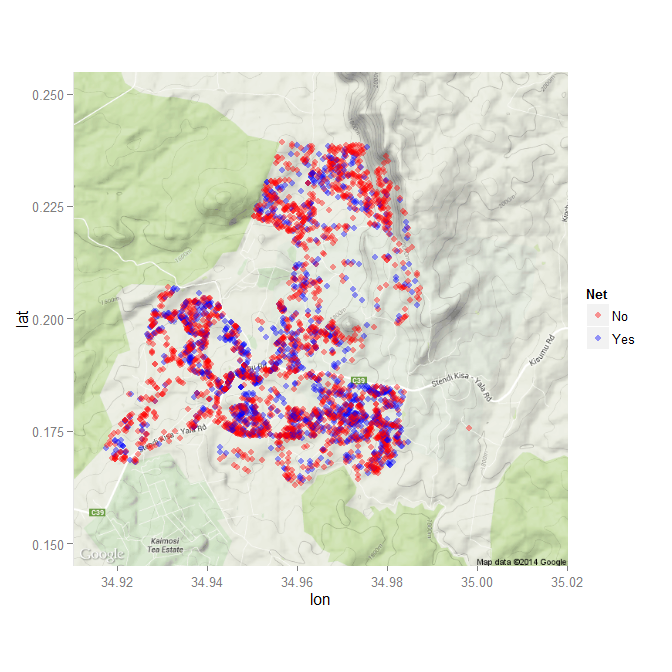
\includegraphics[width=\textwidth]{./figure/High_nets}
\caption{Net usage}
\end{subfigure}
\begin{subfigure}[b]{.48\textwidth}
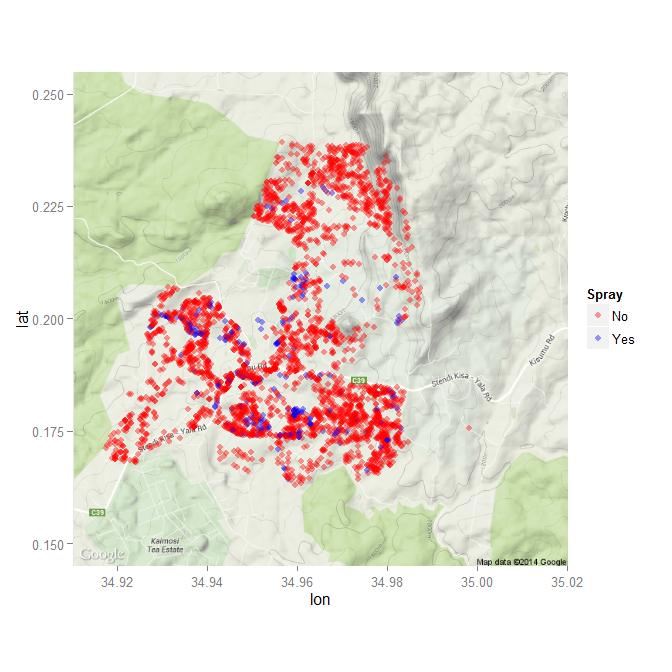
\includegraphics[width=\textwidth]{./figure/High_spray}
\caption{Aerial Spraying}
\end{subfigure}
\caption{The use of bed nets and spraying at the high elevation site.}
\label{high}
\end{figure}

\begin{figure}
\centering
\begin{subfigure}[b]{.48\textwidth}
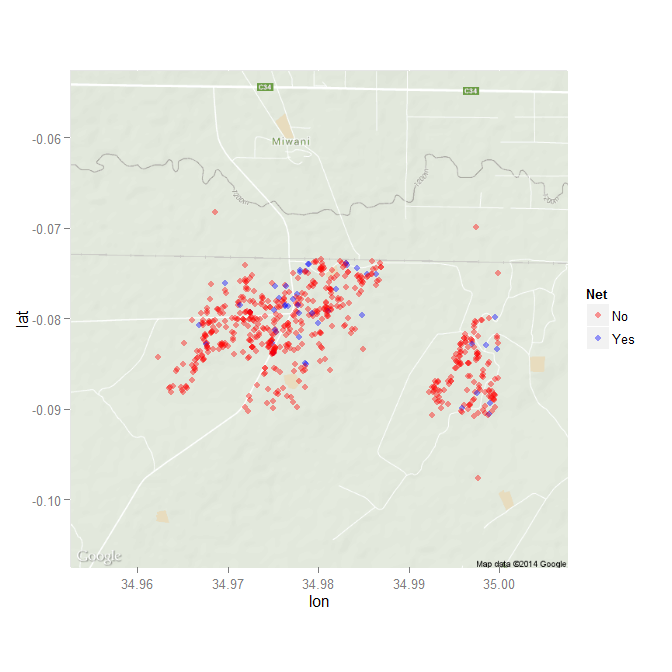
\includegraphics[width=\textwidth]{./figure/Low_nets}
\caption{Net usage}
\end{subfigure}
\begin{subfigure}[b]{.48\textwidth}
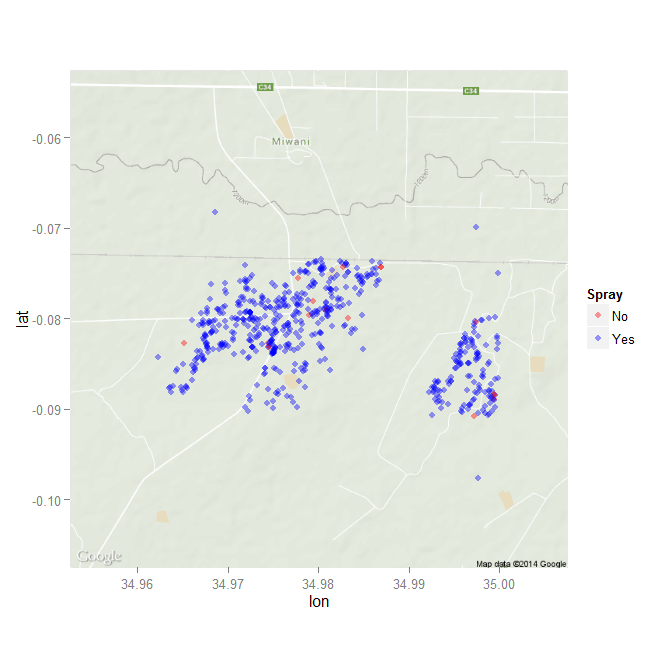
\includegraphics[width=\textwidth]{./figure/Low_spray}
\caption{Aerial Spraying}
\end{subfigure}
\caption{The use of bed nets and spraying at the low elevation site.}
\label{low}
\end{figure}

\FloatBarrier

\subsection{Statistical Methods}
I will use topographical and environmental features to estimate the risk of mosquito exposure for each household.  I will do this by identifying areas where water is likely to pool such as basins, low slope areas, and areas with orthogonal slopes (canyon bottoms).  I will assign each household a risk based on its distance to any of these potential pooling areas.  I will then determine if high risk households are more likely to have received either a bed-net or aerial spraying.\\
Since the two sites have different rates of spraying and net net usage, I will analyze the high and low sites separately.  I will also analyze the spraying and bed net usage separately since these are known to be distributed to households under different protocols.\\


\end{document}
